\documentclass[11pt]{article}
\usepackage[a4paper,margin=2.5cm]{geometry}
\usepackage{fontspec}
\usepackage{xeCJK}
\usepackage{graphicx}
\usepackage{tikz}

% 폰트 설정
\setmainfont{DejaVu Serif}
\setCJKmainfont{Apple SD Gothic Neo}

% 헤더/푸터 제거
\pagestyle{empty}

\begin{document}

% 표지 페이지
\begin{titlepage}
\begin{tikzpicture}[remember picture,overlay]

% 편집 날짜 (오른쪽 상단)
\node[anchor=north east] at ([xshift=-1cm,yshift=-1cm]current page.north east) {
    \footnotesize 25.07.29 편집
};

% 로고 영역 (오른쪽 상단)
\node[anchor=north east] at ([xshift=-1cm,yshift=-3cm]current page.north east) {
    \begin{minipage}{8cm}
        \centering
        % CMS 로고 (실제 파일이 있을 때)
        % 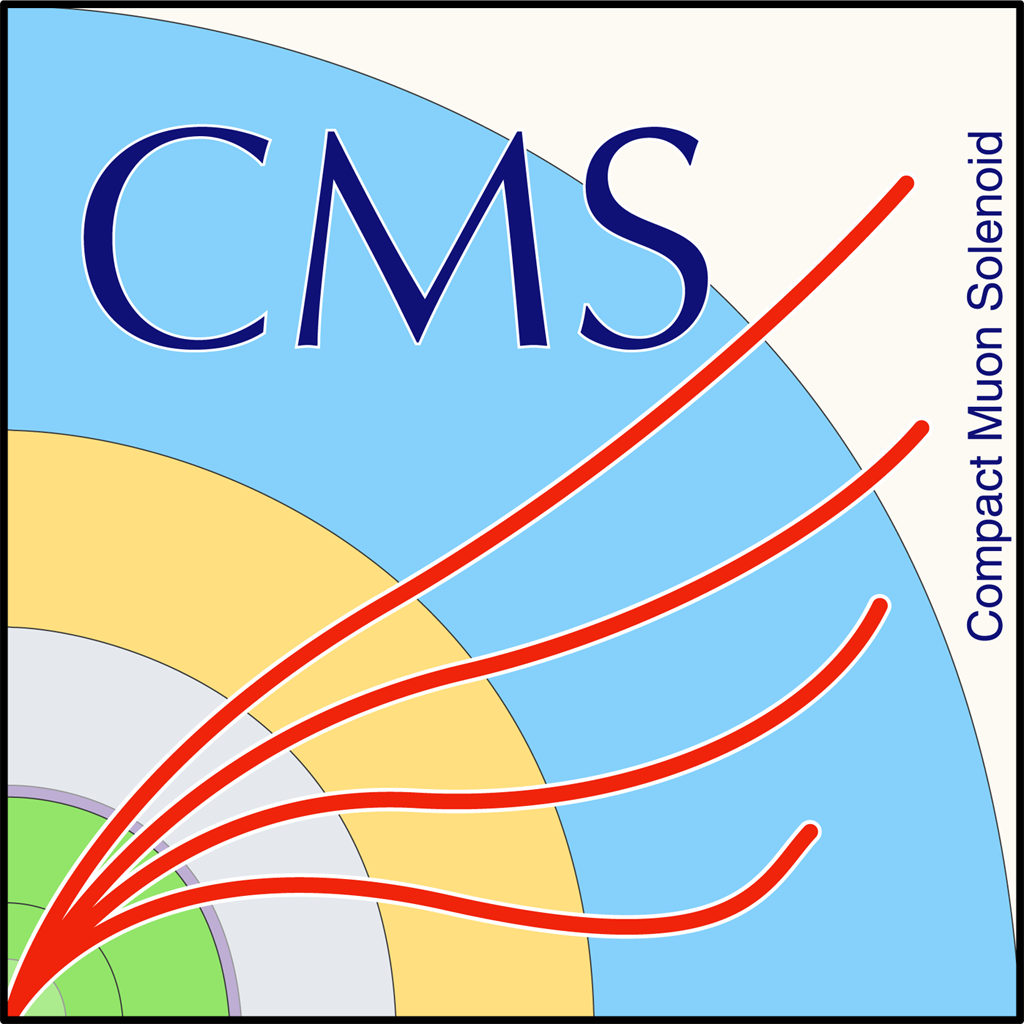
\includegraphics[width=3cm]{cms_logo.png}
        \fbox{\makebox[3cm][c]{\parbox{3cm}{\centering \textbf{CMS}\\EXPERIMENT}}}
        \hspace{0.5cm}
        % 서울대 로고 (실제 파일이 있을 때)
        % 
\includegraphics[width=3cm]{snu_logo.png}
        \fbox{\makebox[3cm][c]{\parbox{3cm}{\centering \textbf{서울대학교}\\SNU}}}
    \end{minipage}
};

% 제목 (중앙)
\node[anchor=center] at (current page.center) {
    \begin{minipage}{15cm}
        \centering
        
        {\Huge\bfseries LRSM WR→tb Channel Analysis}
        
    \end{minipage}
};

\end{tikzpicture}
\end{titlepage}

\end{document}